%%%%%%%%%%%%%%%%%%%%%%%%%%%%%%%%%%%%%%%%%
% Short Sectioned Assignment LaTeX Template Version 1.0 (5/5/12)
% This template has been downloaded from: http://www.LaTeXTemplates.com
% Original author:  Frits Wenneker (http://www.howtotex.com)
% License: CC BY-NC-SA 3.0 (http://creativecommons.org/licenses/by-nc-sa/3.0/)
%%%%%%%%%%%%%%%%%%%%%%%%%%%%%%%%%%%%%%%%%

%----------------------------------------------------------------------------------------
%	PACKAGES AND OTHER DOCUMENT CONFIGURATIONS
%----------------------------------------------------------------------------------------

\documentclass[paper=a4, fontsize=11pt]{scrartcl} % A4 paper and 11pt font size

% ---- Entrada y salida de texto -----

\usepackage{hyperref}
\usepackage{listings}
\usepackage{color}
%AÑADIDO DE LA PÁGINA http://stackoverflow.com/questions/3175105/how-to-insert-code-into-a-latex-doc
\definecolor{dkgreen}{rgb}{0,0.6,0}
\definecolor{gray}{rgb}{0.5,0.5,0.5}
\definecolor{mauve}{rgb}{0.58,0,0.82}

\lstset{frame=tb,
	language=Python,
	aboveskip=3mm,
	belowskip=3mm,
	showstringspaces=false,
	columns=flexible,
	basicstyle={\small\ttfamily},
	numbers=none,
	numberstyle=\tiny\color{gray},
	keywordstyle=\color{blue},
	commentstyle=\color{dkgreen},
	stringstyle=\color{mauve},
	breaklines=true,
	breakatwhitespace=true,
	tabsize=3
}
%%%%%%%%%%%%%%%%%%%%%%%%%%%%%%%%%%%%%%%%%%%%%%%%%%%%%%%
\usepackage{varioref}
\usepackage[T1]{fontenc} % Use 8-bit encoding that has 256 glyphs
\usepackage[utf8]{inputenc}
%\usepackage{fourier} % Use the Adobe Utopia font for the document - comment this line to return to the LaTeX default

% ---- Idioma --------

\usepackage[spanish, es-tabla]{babel} % Selecciona el español para palabras introducidas automáticamente, p.ej. "septiembre" en la fecha y especifica que se use la palabra Tabla en vez de Cuadro

% ---- Otros paquetes ----

\usepackage{amsmath,amsfonts,amsthm} % Math packages
%\usepackage{graphics,graphicx, floatrow} %para incluir imágenes y notas en las imágenes
\usepackage{graphics,graphicx, float} %para incluir imágenes y colocarlas

% Para hacer tablas comlejas
%\usepackage{multirow}
%\usepackage{threeparttable}

%\usepackage{sectsty} % Allows customizing section commands
%\allsectionsfont{\centering \normalfont\scshape} % Make all sections centered, the default font and small caps

\usepackage{fancyhdr} % Custom headers and footers
\pagestyle{fancyplain} % Makes all pages in the document conform to the custom headers and footers
\fancyhead{} % No page header - if you want one, create it in the same way as the footers below
\fancyfoot[L]{} % Empty left footer
\fancyfoot[C]{} % Empty center footer
\fancyfoot[R]{\thepage} % Page numbering for right footer
\renewcommand{\headrulewidth}{0pt} % Remove header underlines
\renewcommand{\footrulewidth}{0pt} % Remove footer underlines
\setlength{\headheight}{13.6pt} % Customize the height of the header

\numberwithin{equation}{section} % Number equations within sections (i.e. 1.1, 1.2, 2.1, 2.2 instead of 1, 2, 3, 4)
\numberwithin{figure}{section} % Number figures within sections (i.e. 1.1, 1.2, 2.1, 2.2 instead of 1, 2, 3, 4)
\numberwithin{table}{section} % Number tables within sections (i.e. 1.1, 1.2, 2.1, 2.2 instead of 1, 2, 3, 4)

\setlength\parindent{0pt} % Removes all indentation from paragraphs - comment this line for an assignment with lots of text

\newcommand{\horrule}[1]{\rule{\linewidth}{#1}} % Create horizontal rule command with 1 argument of height


\renewcommand{\reftextbefore}
	{en la  \reftextvario{página que precede a esta}{página anterior}}
\renewcommand{\reftextafter}
	{en la \reftextvario{siguiente}{siguiente} página}
\renewcommand{\reftextfacebefore}
	{en la  \reftextvario{anterior}{anterior} página}
\renewcommand{\reftextfaceafter}
	{en la \reftextvario{siguiente}{siguiente}{página}}

 \usepackage{algpseudocode}
%----------------------------------------------------------------------------------------
%	TÍTULO Y DATOS DEL ALUMNO
%----------------------------------------------------------------------------------------

\title{	
\normalfont \normalsize 
\textsc{{\bf Algorítmica (2015-2016)} \\ Grado en Ingeniería Informática \\ Universidad de Granada} \\ [25pt] % Your university, school and/or department name(s)
\horrule{0.5pt} \\[0.4cm] % Thin top horizontal rule
\huge Práctica 4-Segunda parte: TSP \\ % The assignment title
\horrule{2pt} \\[0.5cm] % Thick bottom horizontal rule
}

\author{Francisco Carrillo Pérez,Borja Cañavate Bordons, \\Miguel Porcel Jiménez,Jose Manuel Rejón Santiago,Jose Arcos Aneas} % Nombre y apellidos

\date{\normalsize\today} % Incluye la fecha actual

%----------------------------------------------------------------------------------------
% DOCUMENTO
%----------------------------------------------------------------------------------------

\begin{document}

\maketitle % Muestra el Título

\newpage %inserta un salto de página

\tableofcontents % para generar el índice de contenidos

\listoffigures

\listoftables

\newpage
	
	\section{Introducción }

		\begin{itemize}
			\item El objetivo de esta práctica es resolver el problema del TSP utilizando para ello un enfoque Branch and Bound y, alternativamente, otro con Backtracking y comparar ambos.
		\end{itemize}

	
	
	
	%------------------------------------------------
		\section{Representación de la solución} 
		
		
Vector de tamaño N en el que el índice del vector nos indica el orden en el que las ciudades deben de ser visitadas y el contenido de cada posición hace referencia al índice de la ciudad
	
	\section{Diseño del algoritmo: Branch and Bound} 


		
		Usaremos una cola con prioridad que será donde se introduzcan los nodos.
		En la cola se seleccionará el nodo con mayor prioridad, y de dicho nodo se consultará el valor de su cota local, que en caso de ser mejor a la global  y ser nodo hoja, se actualizará la solucion, en caso sólo de ser mejor que la global, se añadiran los hijos del nodo a la cola. En caso de ser peor, se devuelve la solucion actual.
		
		

	\section{Pseudocódigo}
	


		\footnotesize{	
			\begin{algorithmic}				
				\Require Matriz\_costes, Vector\_ciudades[N] Vector\_distancias\_minimas; 
				\State \textbf{Branch\&Bound( Matriz\_costes, Vector\_ciudades Vector\_distancias\_minimas):}
				\State priority\_queue cola;
				\State solucion\_final;
				\State	 Nodo n.generarnodo(Vector\_ciudades[0])
				\While {\textbf{!cola.empty()}}
				\State nodo = cola.top();
				\If{EsHoja(nodo)  \&\& (nodo.cotalocal > cota global ) }
				\State solucion\_final = nodo.solucion;
				\State cota global = nodo.cotalocal;
				\EndIf
				\If{(nodo.cotalocal < cota global )}
				\State cola.add(nodo.generarhijos())
				\State cola.push;
				\Else
				\State return solucion\_final;
				
				\EndIf
				
				\EndWhile
				
				
				
			\end{algorithmic}	
		}

	
	\section{Diseño del algoritmo: Backtracking} 


		
		La solución planteada es el mismo concepto que la aplicada en la anterior práctica, recorreremos el árbol en profundidad, calculando en cada nodo el valor de la cota local salvo que en caso de ser mayor que la global, podamos (ignoramos) a ese nodo y a todos sus hijos.
		
		

	\section{Pseudocódigo}


		\footnotesize{	
			\begin{algorithmic}				
				\Require Matriz, S\_final[N] S\_parcial[N] Ciudades[N]={false} ciudad\_actual, nivel,valor\_maximo=0;
				\State \textbf{Backtrack(S,S\_parcial,Ciudades,ciudad\_actual,nivel):}
				\State Ciudades[ciudad\_actual]=true;
				\State	   S\_parcial[nivel - 1]=ciudad\_actual;
				\For {\textbf{i} to \textbf{N}}
				
				\If {Ciudades[i]==false}
				\State 	valor\_actual = CalcularSolucionActual(S\_parcial);
				\If {(cotalocal < cotaglobal)}
				\State 	\textbf{Backtrack(S,S\_parcial,Ciudades,i,nivel+1);}
				\EndIf
				\If{nodo\_actual == nodo\_hoja}
				\State{ valor\_actual = CalcularSolucionActual(S\_parcial)}
				\If{valor\_actual \textbf{mayor que} valor\_maximo}
				\State{ S\_final = S\_Actual}
				\State{ valor\_maximo = valor\_actual}
				\EndIf
				\EndIf
				
				\State Ciudades[i] = false;
				\EndIf
				\EndFor
			\end{algorithmic}			
		}

	
	
	\section{Comparación}


		En ambos programas, hemos analizado los mismos mapas. Compararemos los tiempos y el empleo de los nodos para cada tipo de técnica empleada

	
	


		\begin{figure}[H]
			\centering
			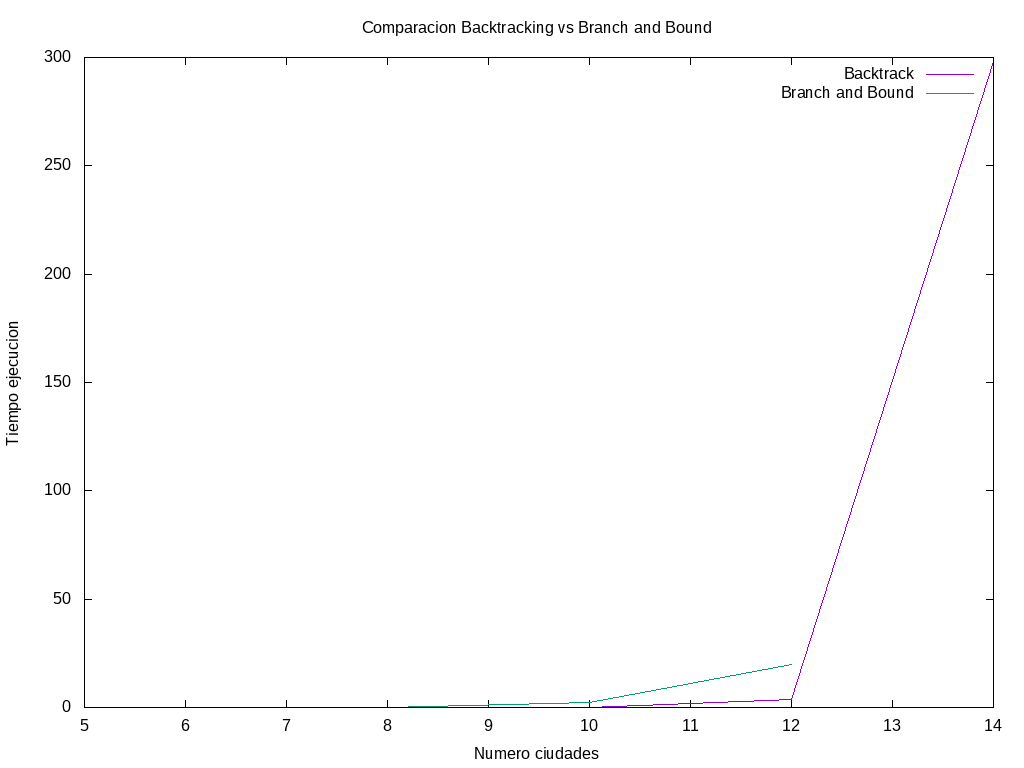
\includegraphics[width=0.7\linewidth]{../Codigo/Solucion/comparacion}
			\caption{comparacion entre ambos }
			\label{fig:comparacion}
		\end{figure}
		
		

	
	



		\begin{table}[H]
							Mapa ulysses 5
			\centering
			
			\label{my-label}
			\begin{tabular}{lllll}
				Técnica	& Branch and bound & Backtracking  &   \\
				N.totales& 120&120  &  &  \\
				N.podados&  35& 68 &  &  \\
				N.explorados&85  &52  &  &  \\
				
			\end{tabular}
		\end{table}
		

	
	



		\begin{table}[H]
			Mapa ulysses 8
			\centering
			
			\label{my-label}
			\begin{tabular}{lllll}
				Técnica	& Branch and bound & Backtracking  &   \\
				N.totales& 40320&40320  &  &  \\
				N.podados&  38568& 37605 &  &  \\
				N.explorados&1752  &2715 &  &  \\
				
			\end{tabular}
		\end{table}
		

	
	


 
		\begin{table}[H]
							Mapa ulysses 10
			\centering
			
			\label{my-label}
			\begin{tabular}{lllll}
				Técnica	& Branch and bound & Backtracking  &   \\
				N.totales& 3628800&3628800  &  &  \\
				N.podados&  3601453& 3566077 &  &  \\
				N.explorados&27347  &62723  &  &  \\
				
			\end{tabular}
		\end{table}
		

	
	

	
						
		\begin{table}[H]
			Mapa ulysses 12
			\centering
			
			\label{my-label}
			\begin{tabular}{lllll}
				Técnica	& Branch and bound & Backtracking  &   \\
				N.totales& 479001600&479001600 &  &  \\
				N.podados&  478284703& 474474230&  &  \\
				N.explorados&716897  &4527370  &  &  \\
				
			\end{tabular}
		\end{table}
		

	


\end{document}